\documentclass[conference]{IEEEtran}
\IEEEoverridecommandlockouts
\usepackage[utf8]{inputenc}
\usepackage[T1]{fontenc}
\usepackage[spanish,es-noshorthands,es-tabla]{babel}
\usepackage{cite}
\usepackage{amsmath,amssymb}
\usepackage{graphicx}
\usepackage{booktabs}
\usepackage{url}
\usepackage[hidelinks]{hyperref}
\graphicspath{{fig/}}

\begin{document}

\title{TRM Predict: analítica predictiva en la nube para el riesgo cambiario en Colombia\\
{\large Avance del proyecto integrador: Minería de Datos, Cloud Computing y Machine Learning}}

\author{
\IEEEauthorblockN{Sebastián Cubides, Nicolás Vergara, Edgar Ruiz}
\IEEEauthorblockA{\textit{Ingeniería de Datos e Inteligencia Artificial, V semestre}\\
\textit{Universidad Santo Tomás}, Tunja, Colombia\\
Proyecto integrador: Minería de Datos, Machine Learning y Cloud Computing --- 2026-2}
}

\maketitle

\begin{abstract}
Este documento presenta el avance de \emph{TRM Predict}, una plataforma en la nube que estima para el siguiente día hábil si la TRM subirá, cuál será su valor esperado y qué probabilidad hay de un movimiento fuerte. Se cubre el planteamiento del problema y su relación con los ODS~8 y~10, la construcción y limpieza de un dataset de 2.159 días hábiles y 43 variables, el análisis exploratorio, el módulo de web scraping de noticias y la minería no supervisada (K-Means, DBSCAN y reglas de asociación). En infraestructura se describe el despliegue en AWS con Terraform, las pruebas de disponibilidad y de carga, la recuperación ante desastres y la estimación preliminar de costos (63,6~USD al mes encendido de forma continua, cerca de 21~USD para el semestre). Por último se integra el módulo de Machine Learning: de 19 modelos optimizados solo los ensembles superan las líneas base fuera de muestra (ROC-AUC de 0,566 en dirección y 0,586 en riesgo). Todo el código es reproducible y está en \url{https://github.com/Sebas-409/proyecto-integrador-trm}.
\end{abstract}

\begin{IEEEkeywords}
computación en la nube, minería de datos, machine learning, AWS, Terraform, CRISP-DM, clustering, reglas de asociación, tasa de cambio, desarrollo sostenible
\end{IEEEkeywords}

\section{Introducción}
La \emph{Tasa Representativa del Mercado} (TRM) es la tasa de cambio oficial entre el peso colombiano y el dólar, y la certifica cada día hábil la Superintendencia Financiera. De ella dependen el precio de los bienes importados, el valor de las remesas que reciben los hogares y el costo de la deuda en dólares. Entre septiembre de 2017 y octubre de 2026 se movió entre 2.705 y 5.061 pesos por dólar, y en el 18~\% de las jornadas la variación diaria fue superior al 1~\%.

Las grandes empresas manejan ese riesgo con mesas de tesorería y coberturas con derivados. En cambio, los hogares que reciben remesas y las mipymes importadoras suelen decidir por intuición cuándo cambiar sus divisas. Las remesas hacia Colombia superaron los 11.800 millones de dólares en 2024~\cite{banrep_remesas}, así que elegir mejor el día de cambio tiene un efecto directo en el ingreso de las familias.

Este avance sigue la estructura modular de los lineamientos: documento técnico (Secciones I a III), módulo de Minería de Datos (Sección IV), módulo de Cloud Computing (Sección V) e integración con Machine Learning (Sección VI).

\section{Planteamiento del problema y ODS}
\textbf{Usuarios.} Hogares que reciben remesas, mipymes importadoras y programas de educación financiera.

\textbf{Pregunta.} Usando solo información pública disponible antes de que se certifique la TRM del día siguiente, ¿es posible anticipar (a) su dirección, (b) su valor esperado y (c) la ocurrencia de un movimiento brusco, mejor que un paseo aleatorio? La pregunta no es trivial: Meese y Rogoff mostraron que los modelos estructurales de tasa de cambio no superan a un paseo aleatorio fuera de muestra~\cite{meese1983}. Por eso el paseo aleatorio y la clase mayoritaria son las líneas base obligatorias del proyecto.

\textbf{Vínculo con los ODS.} Dentro de la Agenda 2030~\cite{un2015}, el proyecto aporta a la meta 8.10 del ODS~8 (acceso a servicios financieros), porque acerca analítica cambiaria a pequeñas empresas que no pueden pagar asesoría especializada, y a la meta 10.c del ODS~10 (reducir el costo de las remesas), porque una mejor ventana de cambio mejora el ingreso real de los hogares.

\textbf{Trabajos relacionados.} Las revisiones de Henrique \emph{et al.}~\cite{henrique2019} y Sezer \emph{et al.}~\cite{sezer2020} muestran que la mayoría de estudios trabaja con monedas principales o índices bursátiles y se queda en la evaluación fuera de línea. Este proyecto se enfoca en una moneda emergente, usa determinantes propios del país y entrega un servicio desplegado y reproducible.

\section{Estructura general del sistema}
La solución tiene tres bloques desacoplados (Fig.~\ref{fig:arch}). Primero, un flujo diario de ingesta y minería que reúne la TRM oficial, series de mercado, criptoactivos y titulares de prensa. Segundo, un entorno de entrenamiento fuera de línea que genera y versiona los modelos de Machine Learning. Tercero, una API en contenedores detrás de un balanceador en AWS que sirve las predicciones y el tablero web de consulta.

\begin{figure*}[t]
\centering
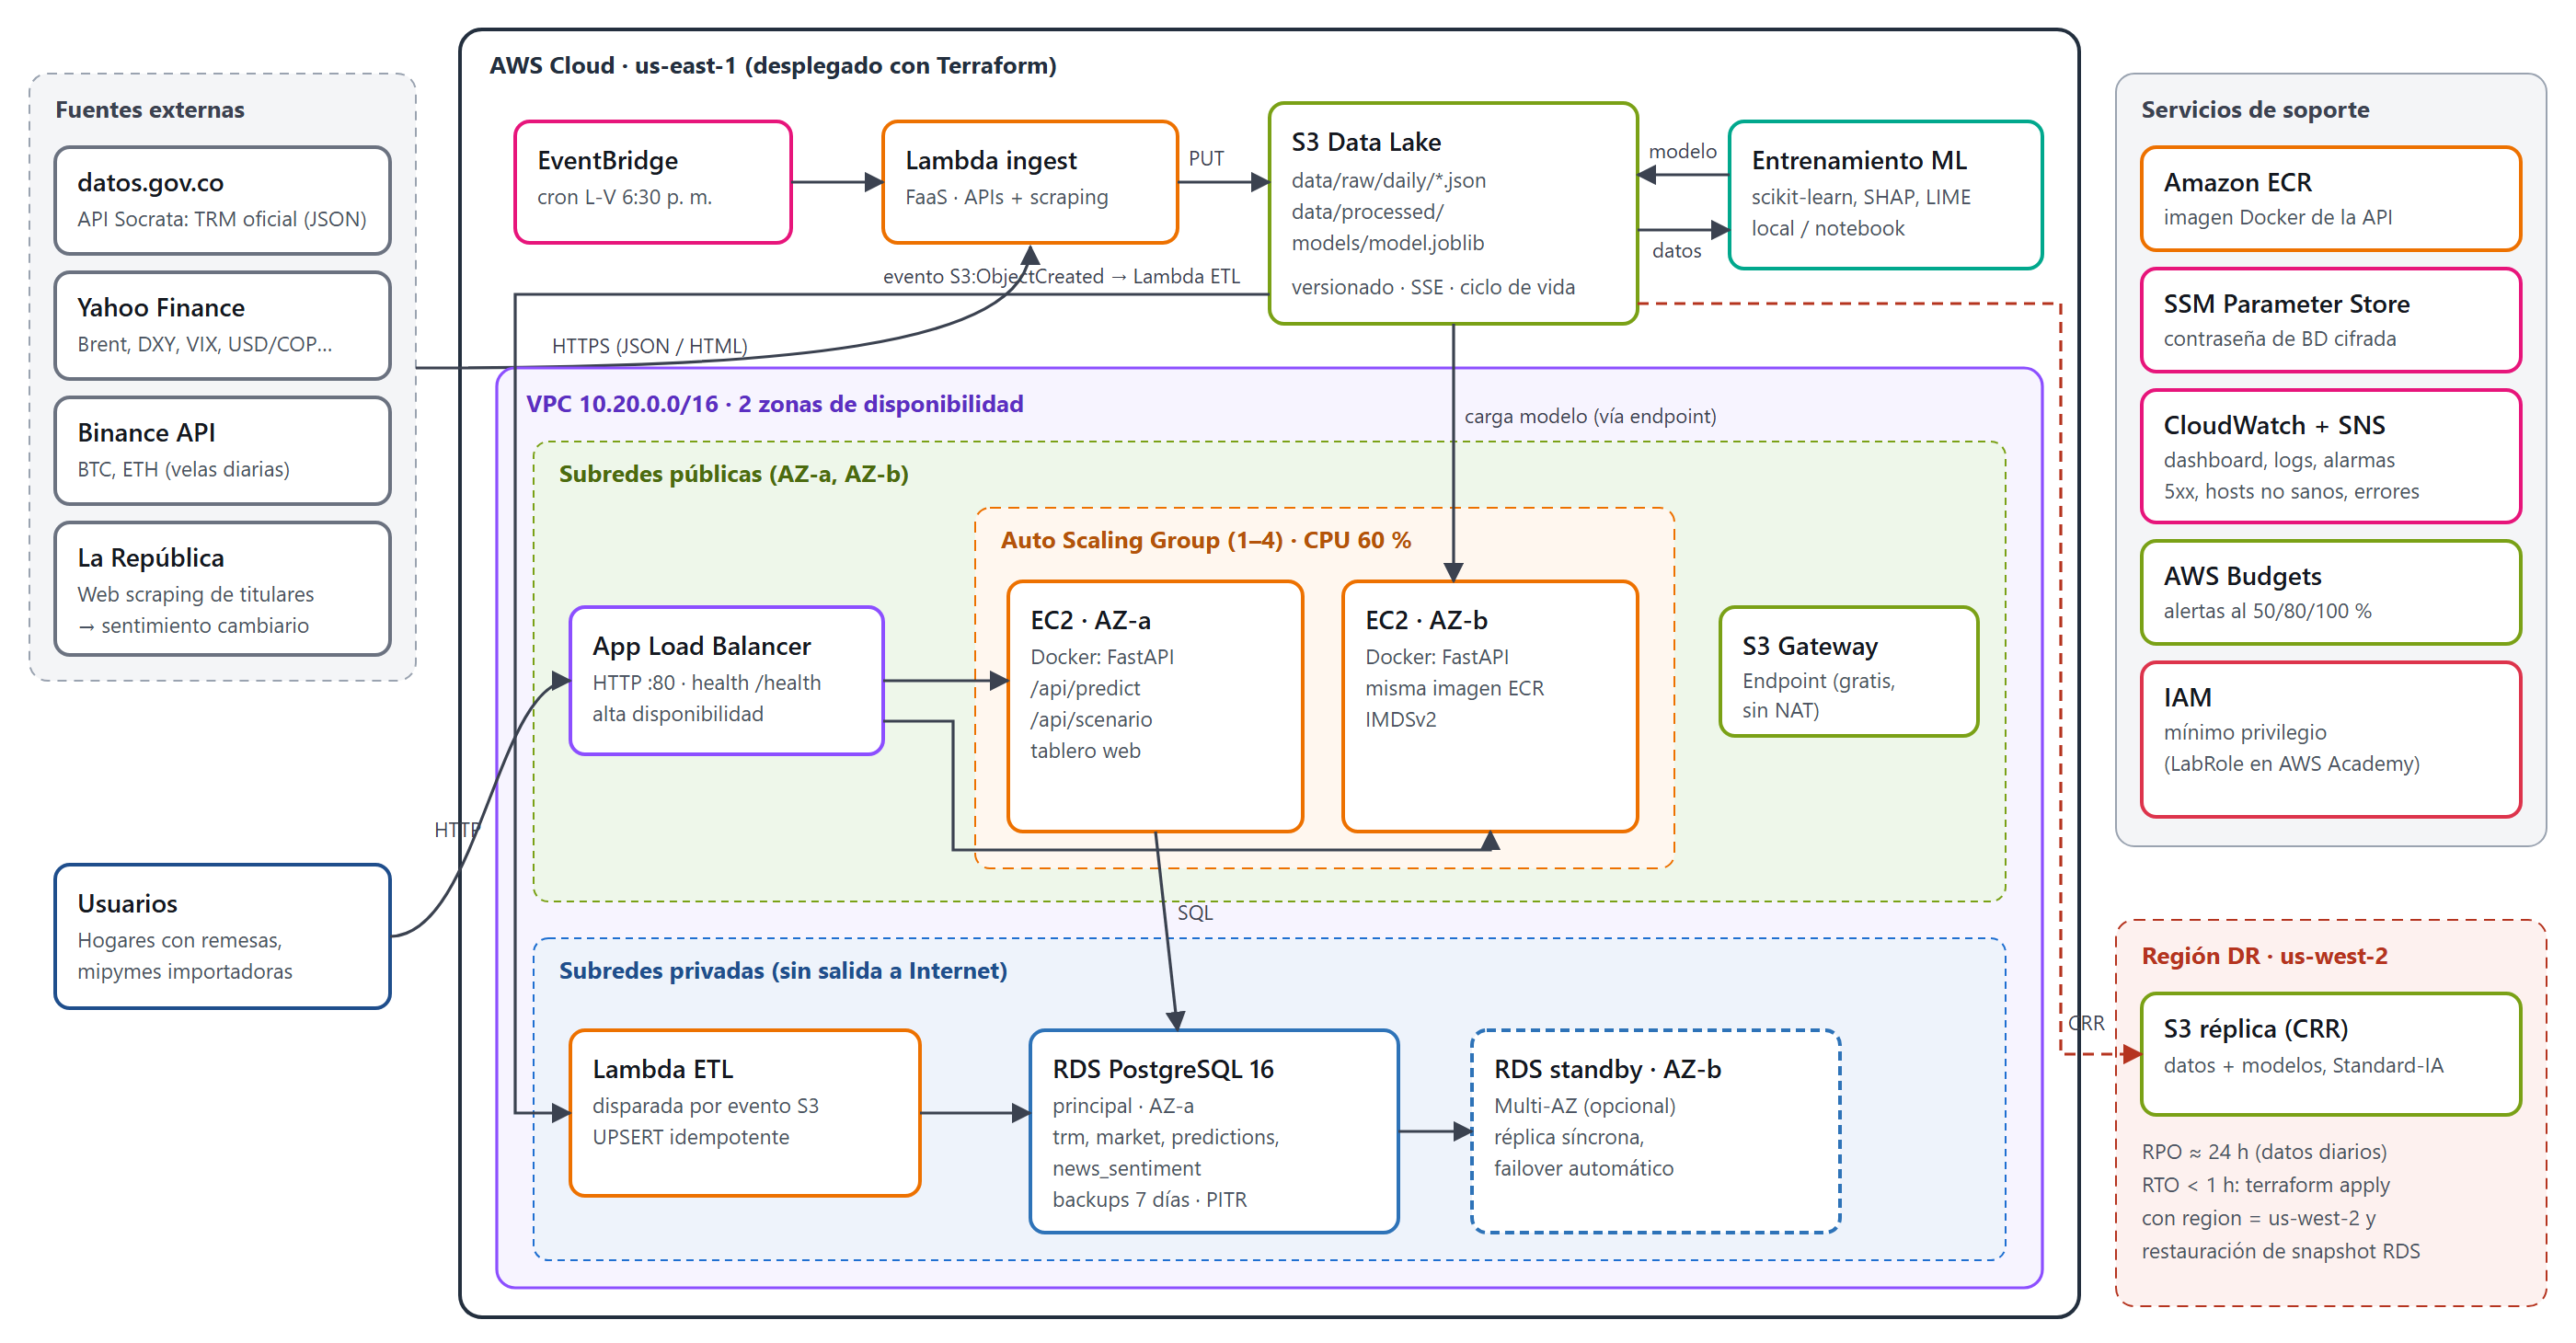
\includegraphics[width=0.92\textwidth]{arquitectura.png}
\caption{Arquitectura de TRM Predict en AWS, aprovisionada con Terraform.}
\label{fig:arch}
\end{figure*}

\section{Módulo de Minería de Datos}
El procesamiento sigue las etapas del proceso KDD~\cite{fayyad1996} organizadas con CRISP-DM~\cite{wirth2000}. Cada etapa es un módulo de Python que se ejecuta de principio a fin.

\subsection{Dataset estructurado y prevención de fuga de datos}
La tabla maestra (\texttt{data/processed/dataset.csv}, construida con \texttt{src/pipeline/prepare.py}) reúne 2.159 días hábiles entre el 7 de septiembre de 2017 y el 17 de octubre de 2026, con 43 variables explicativas. La fecha de inicio la define la disponibilidad de cotizaciones diarias de Bitcoin y Ethereum. Para evitar cualquier filtración de datos del futuro, las series de distintos husos horarios se cruzaron con \texttt{merge\_asof} sin coincidencias exactas, de modo que cada registro solo incorpora cierres ocurridos antes de la publicación de la TRM objetivo. Las Tablas~\ref{tab:sources} y~\ref{tab:vars} detallan las fuentes y las variables.

\begin{table}[t]
\caption{Fuentes de datos externas y formatos de ingesta}
\label{tab:sources}
\centering
\footnotesize
\begin{tabular}{@{}p{2.0cm}p{1.4cm}p{4.0cm}@{}}
\toprule
Fuente & Tipo & Contenido \\
\midrule
datos.gov.co (Superfinanciera) & API, JSON & TRM oficial diaria desde 1991 (8.370 registros) \\
Yahoo Finance & API, JSON a CSV & Brent, DXY, bono a 10 años de EE.~UU., VIX, S\&P~500, USD/MXN, USD/BRL y dólar spot USD/COP (entre 4.786 y 5.156 registros por serie) \\
Binance & API, JSON a CSV & Precio diario de cierre de BTC y ETH (3.352 registros por serie) \\
La República & Scraping HTML & Titulares económicos e índice diario de sentimiento del dólar \\
\bottomrule
\end{tabular}
\end{table}

\begin{table}[t]
\caption{Grupos de variables del dataset final}
\label{tab:vars}
\centering
\footnotesize
\begin{tabular}{@{}p{1.9cm}p{5.7cm}@{}}
\toprule
Grupo & Variables \\
\midrule
TRM & Retornos de los 5 días anteriores, retorno a 5 días, volatilidad a 5 y 20 días, razón de medias móviles y z-score a 20 días \\
Calendario & Día de la semana y mes \\
Mercados (10 series) & Retorno a 1 día, retorno a 5 días y volatilidad a 20 días de cada serie \\
Brecha spot--TRM & Diferencia porcentual entre el dólar spot y la TRM vigente \\
Objetivos & Retorno del día siguiente (\texttt{y\_ret}) y dirección binaria de subida (\texttt{y\_up}) \\
\bottomrule
\end{tabular}
\end{table}

\subsection{Manejo de nulos y outliers}
El control de calidad queda registrado en \texttt{reports/data\_quality.json}. En la limpieza se estandarizaron formatos de fecha y número, se eliminaron registros duplicados o vacíos y se comprobó que ninguna serie tuviera precios iguales o menores a cero (no apareció ningún caso). Al descartar las primeras filas, que quedan incompletas por el cálculo de rezagos y ventanas móviles de 20 días, la matriz final queda con 0 valores nulos.

Para los valores extremos se identificaron los retornos diarios que superan tres veces el rango intercuartílico (Tabla~\ref{tab:outliers}). Como esos picos son episodios reales de tensión financiera, se conservaron para los modelos supervisados basados en árboles, que son robustos a ellos. Para el agrupamiento no supervisado sí fue necesario acotar las colas en los percentiles 1 y 99 (44 datos por variable), porque sin ese ajuste K-Means dedicaba grupos enteros a aislar las caídas abruptas de 2020.

\begin{table}[t]
\caption{Retornos atípicos por serie (regla de $3\times$IQR)}
\label{tab:outliers}
\centering
\footnotesize
\begin{tabular}{@{}lrlr@{}}
\toprule
Serie & Atípicos & Serie & Atípicos \\
\midrule
S\&P 500 & 99 & Bono a 10 años & 44 \\
USD/COP spot & 82 & VIX & 44 \\
BTC & 63 & USD/MXN & 41 \\
Brent & 61 & USD/BRL & 38 \\
ETH & 48 & DXY & 16 \\
\bottomrule
\end{tabular}
\end{table}

\subsection{Análisis Exploratorio de Datos (EDA)}
Las pruebas descriptivas (\texttt{src/pipeline/eda.py}) confirman el comportamiento típico de los activos financieros (Tabla~\ref{tab:desc} y Fig.~\ref{fig:serie}). El retorno diario promedia apenas 0,004~\%, tiene asimetría positiva (0,50) y un exceso de curtosis de 2,99, es decir, colas más pesadas que una distribución normal; la prueba de Jarque--Bera rechaza la normalidad con un valor $p$ prácticamente nulo (Fig.~\ref{fig:hist}).

Ninguna variable supera por sí sola una correlación lineal de 0,17 con el retorno del día siguiente (Tabla~\ref{tab:corr} y Fig.~\ref{fig:corr}). Además, en ventanas móviles de 120 días frente al Brent, el DXY y el Bitcoin, el signo de la correlación cambia según la coyuntura (Fig.~\ref{fig:roll}), por lo que los modelos lineales resultan insuficientes.

\begin{table}[t]
\caption{Estadísticas descriptivas del retorno diario de la TRM}
\label{tab:desc}
\centering
\footnotesize
\begin{tabular}{@{}lr@{}}
\toprule
Estadística & Valor \\
\midrule
Media & 0,004~\% \\
Desviación estándar & 0,81~\% \\
Asimetría & 0,50 \\
Curtosis en exceso & 2,99 \\
Autocorrelación con el día anterior & 0,17 \\
Días en que sube & 48,3~\% \\
\bottomrule
\end{tabular}
\end{table}

\begin{table}[t]
\caption{Correlación lineal con el retorno del día siguiente}
\label{tab:corr}
\centering
\footnotesize
\begin{tabular}{@{}lr@{}}
\toprule
Variable & Correlación \\
\midrule
Retorno de la TRM del día anterior & 0,17 \\
Retorno del Brent a 1 día & 0,13 \\
Retorno del Brent a 5 días & 0,11 \\
Retorno del DXY a 1 día & 0,09 \\
Retorno del S\&P 500 a 1 día & 0,09 \\
Retorno del VIX a 1 día & 0,08 \\
\bottomrule
\end{tabular}
\end{table}

\begin{figure}[t]
\centering
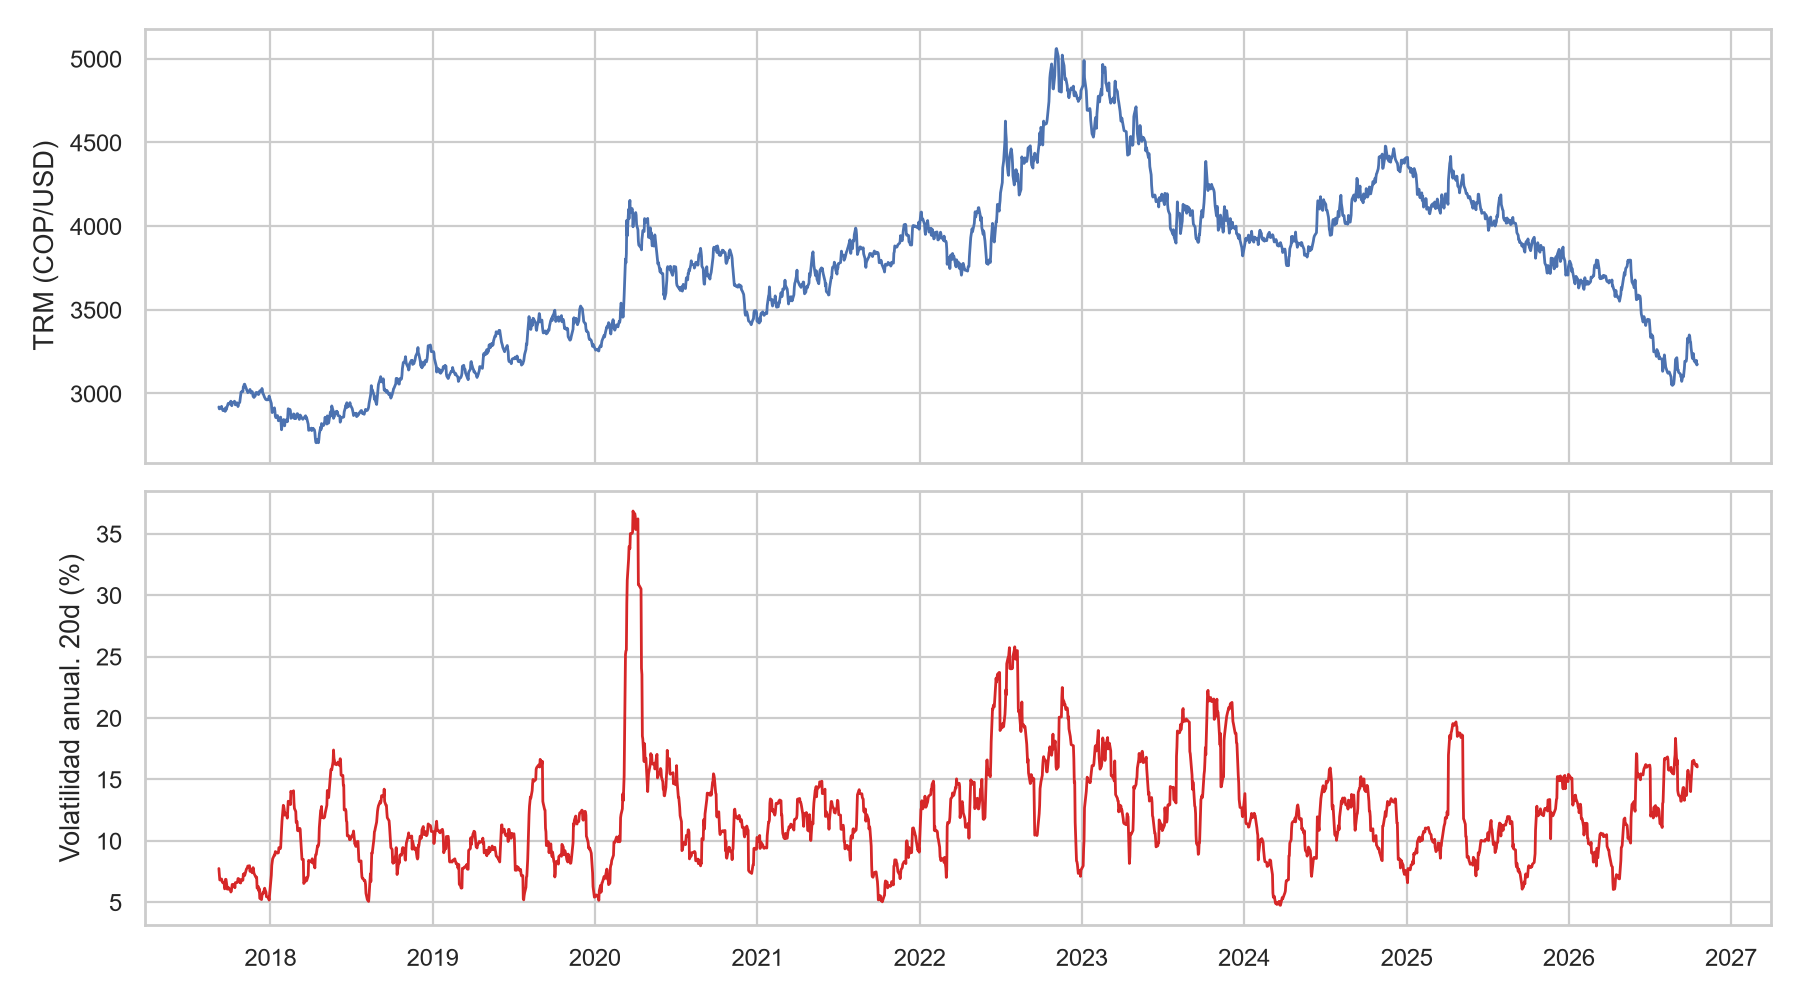
\includegraphics[width=\columnwidth]{eda_trm_series.png}
\caption{Serie histórica de la TRM y volatilidad móvil a 20 días.}
\label{fig:serie}
\end{figure}

\begin{figure}[t]
\centering
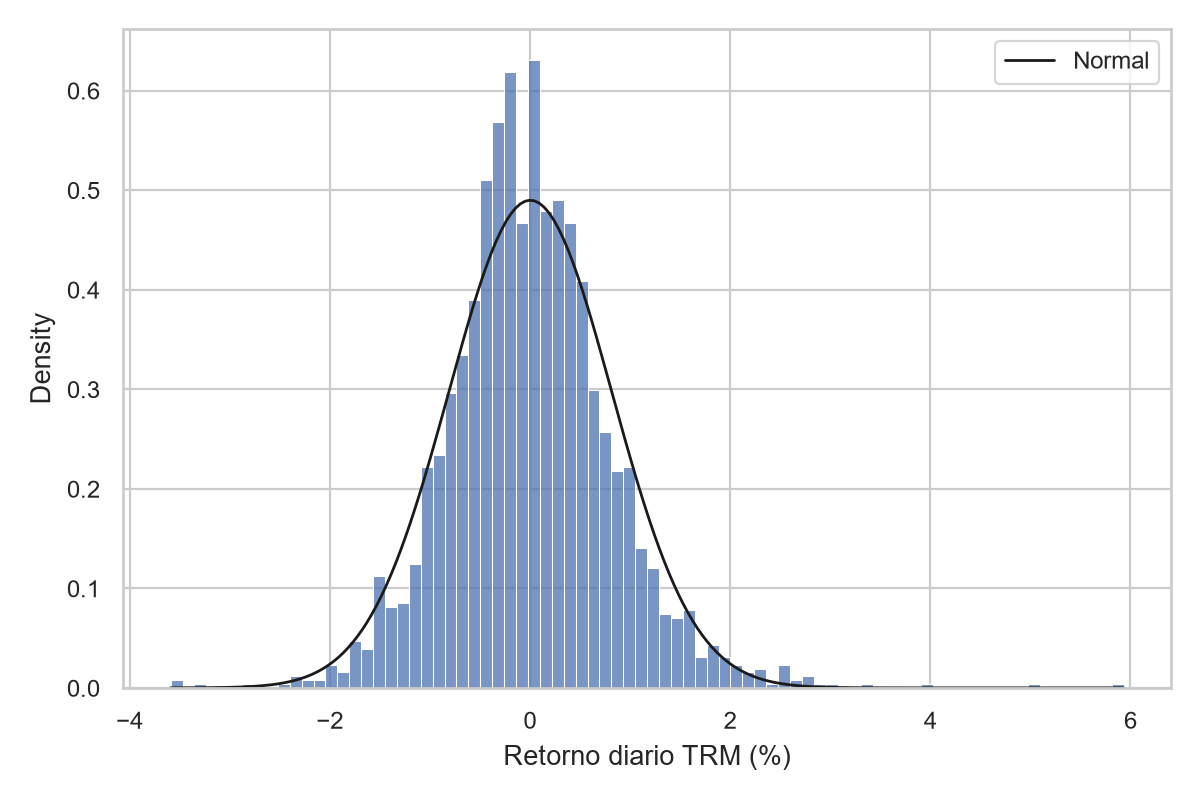
\includegraphics[width=0.9\columnwidth]{eda_returns_hist.png}
\caption{Distribución empírica de los retornos diarios de la TRM.}
\label{fig:hist}
\end{figure}

\begin{figure}[t]
\centering
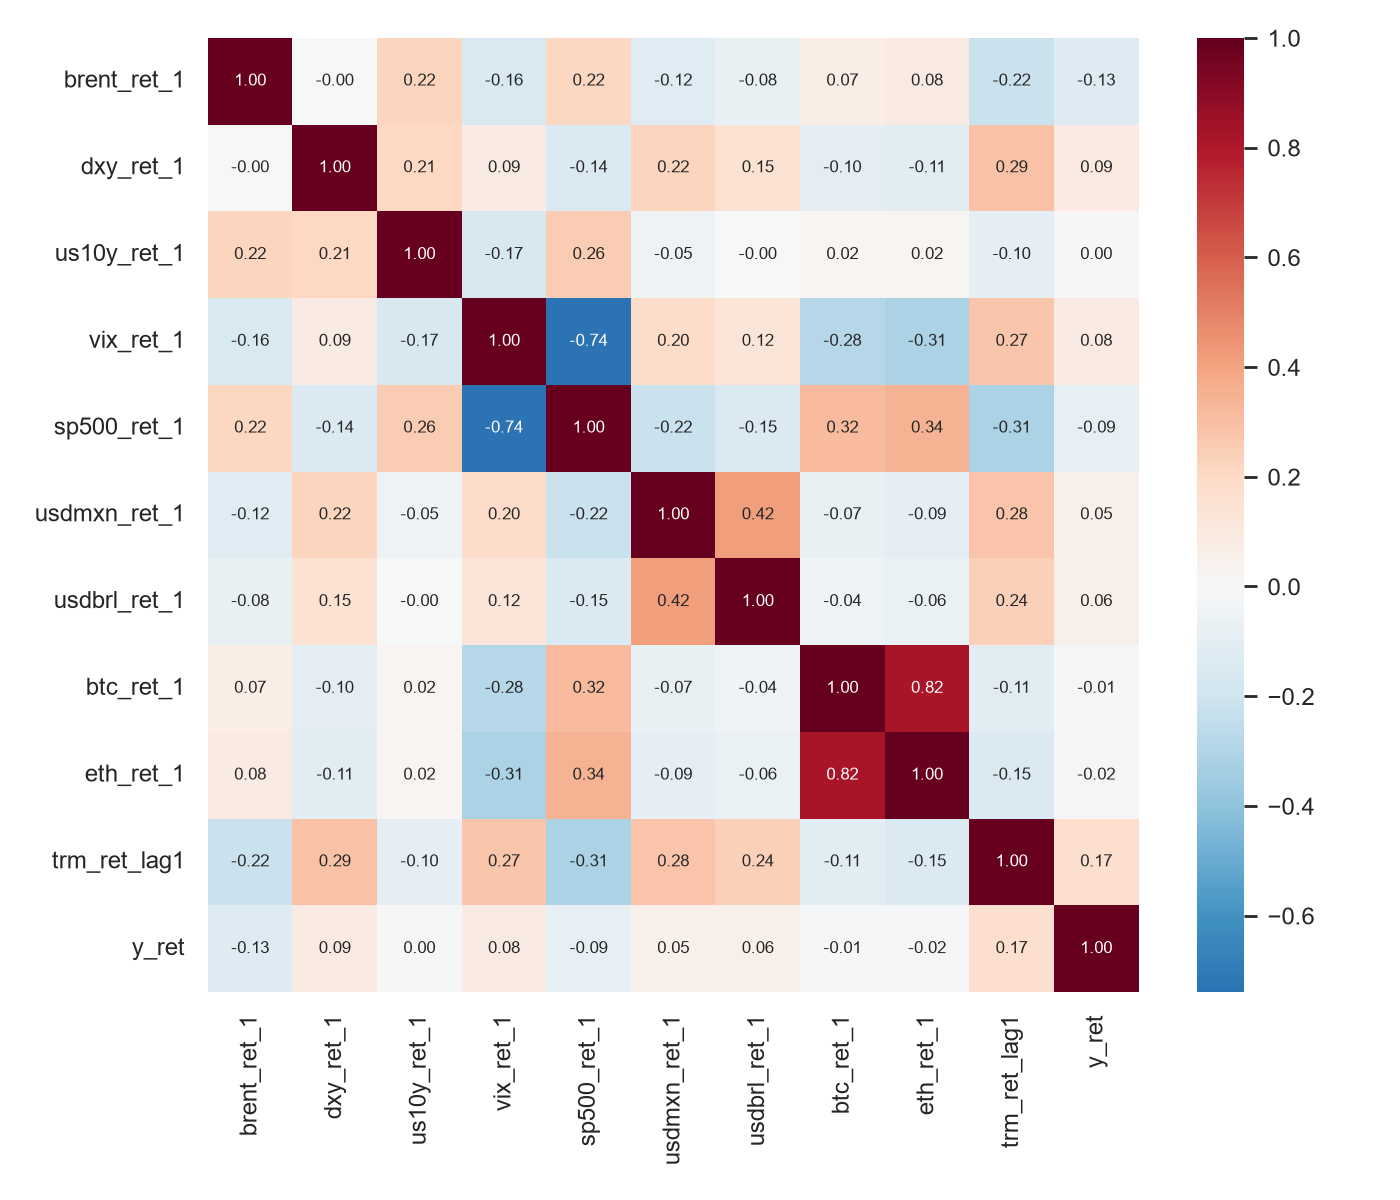
\includegraphics[width=\columnwidth]{eda_corr.png}
\caption{Matriz de correlación entre variables explicativas.}
\label{fig:corr}
\end{figure}

\begin{figure}[t]
\centering
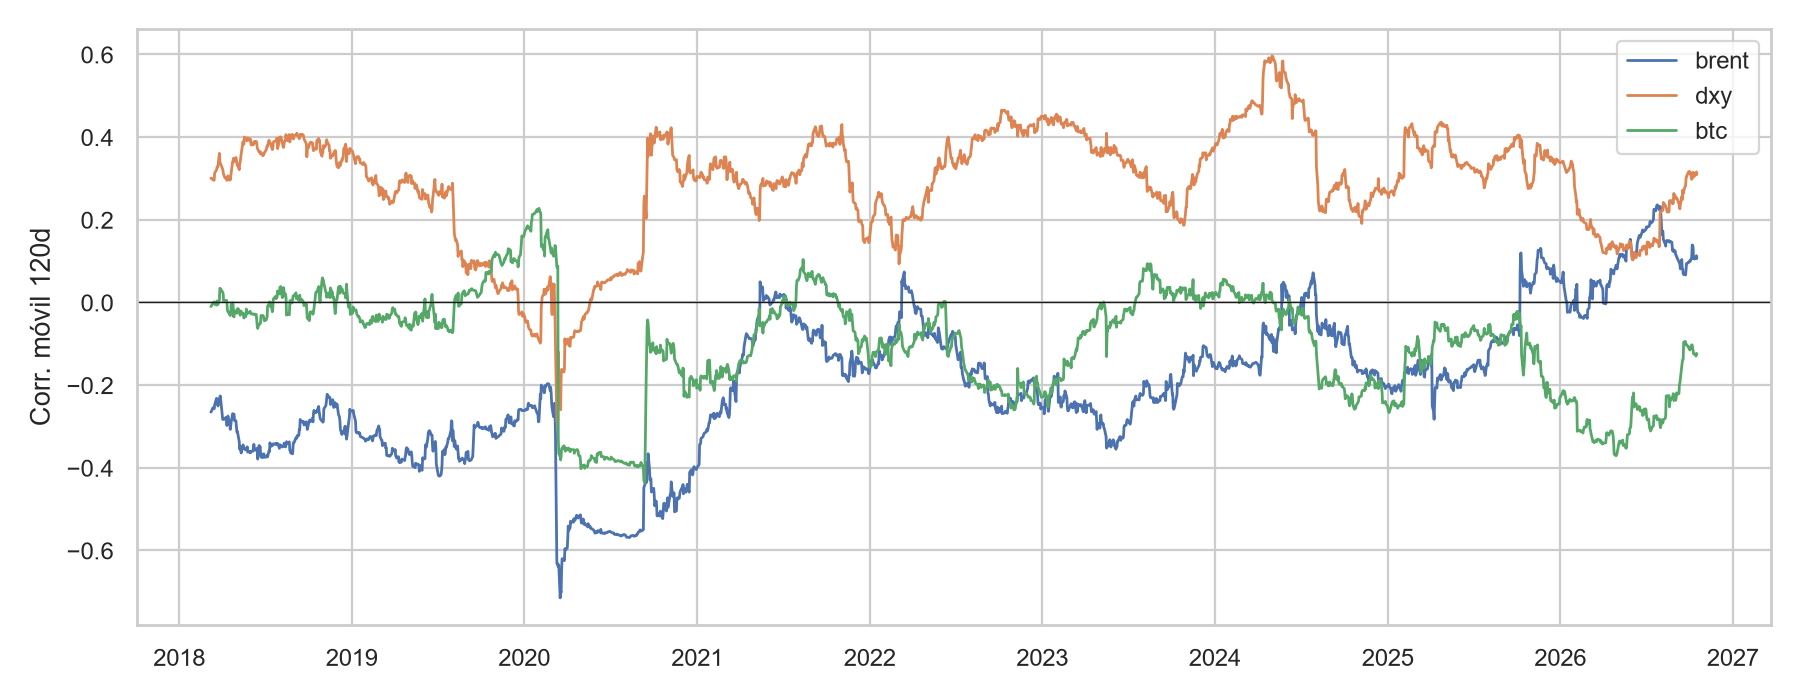
\includegraphics[width=\columnwidth]{eda_rolling_corr.png}
\caption{Correlación móvil a 120 días entre la TRM y el Brent, el DXY y el BTC.}
\label{fig:roll}
\end{figure}

\subsection{Módulo de Web Scraping y fuentes externas}
Las cotizaciones no recogen por sí solas el tono de la coyuntura local. Por eso se programó \texttt{src/ingest/scraper.py}, que lee a diario los titulares de las secciones Finanzas, Economía y Globoeconomía del diario \emph{La República}. El código usa únicamente \texttt{html.parser} de la biblioteca estándar de Python para poder empaquetarse sin dependencias pesadas dentro de AWS Lambda, hace una sola consulta diaria por sección respetando \texttt{robots.txt} y extrae los enlaces dentro de las etiquetas \texttt{h2} y \texttt{h3}.

Con esos textos se calculan dos indicadores diarios: \texttt{n\_titulares\_dolar}, que cuenta las menciones al dólar o a la TRM, y \texttt{sentimiento\_dolar}, una escala entre $-1$ y $1$ que pondera términos de presión alcista (sube, devaluación, incertidumbre) frente a bajista (cae, revaluación, fortalece). En la ejecución guardada en \texttt{data/raw/news/sentiment\_2026-10-20.json}, de 79 titulares recolectados, 2 trataban sobre el dólar y dieron un índice neto de $-0{,}64$. Como el medio no tiene hemeroteca abierta, los registros se acumulan día a día en S3 y se muestran en el tablero como referencia mientras reúnen historia suficiente para entrar al entrenamiento. Las demás fuentes externas (datos.gov.co, Yahoo Finance y Binance) se consumen por API en \texttt{src/ingest/apis.py}.

\subsection{Minería no supervisada}
En \texttt{src/pipeline/unsupervised.py} y \texttt{src/pipeline/elbow.py} se aplicaron algoritmos de agrupamiento y de reglas de asociación.

\subsubsection{Clustering y regímenes de mercado}
Para describir el estado del mercado se tomaron 9 variables estandarizadas de volatilidad y retorno a 5 días, y se probó K-Means con $k$ entre 1 y 10. El codo de la curva de inercia (Fig.~\ref{fig:codo}) sugiere $k=4$ regímenes (Tabla~\ref{tab:regimes}). El coeficiente de silueta es un poco mayor con $k=3$ (0,122 frente a 0,116 con $k=4$, índice de Davies--Bouldin de 1,91), tanto en K-Means como en el método jerárquico de Ward, pero con cuatro grupos se separan los episodios de crisis (2,2~\% de la muestra), en los que la desviación del retorno del día siguiente sube hasta 1,47~\%. La silueta baja indica que los regímenes se traslapan, por lo que se usan como contexto y no como clases rígidas.

DBSCAN~\cite{ester1996} ($\varepsilon=2{,}89$, \texttt{min\_samples}=18) se ejecutó sobre la serie sin recortar colas para detectar jornadas anómalas. El algoritmo aisló 57 días atípicos, 45 de ellos en 2020, en los que la volatilidad posterior llega a 1,38~\%, casi el doble del 0,79~\% de las jornadas normales. El análisis de componentes principales (PCA) necesita 26 de las 43 dimensiones para conservar el 90~\% de la varianza, así que la redundancia entre variables es baja y la proyección en dos dimensiones se usa solo con fines gráficos (Fig.~\ref{fig:pca}).

\begin{table}[t]
\caption{Regímenes de mercado de K-Means ($k=4$) y comportamiento del día siguiente}
\label{tab:regimes}
\centering
\footnotesize
\begin{tabular}{@{}p{2.9cm}rrrr@{}}
\toprule
Régimen & Días & \% días & TRM sube & $\sigma$ ret. sig. \\
\midrule
Calma & 752 & 34,8~\% & 50,8~\% & 0,63~\% \\
Apetito por riesgo (peso se aprecia) & 754 & 34,9~\% & 43,8~\% & 0,84~\% \\
Aversión al riesgo (dólar sube) & 606 & 28,1~\% & 51,3~\% & 0,90~\% \\
Crisis o alta volatilidad & 47 & 2,2~\% & 42,6~\% & 1,47~\% \\
\bottomrule
\end{tabular}
\end{table}

\begin{figure}[t]
\centering
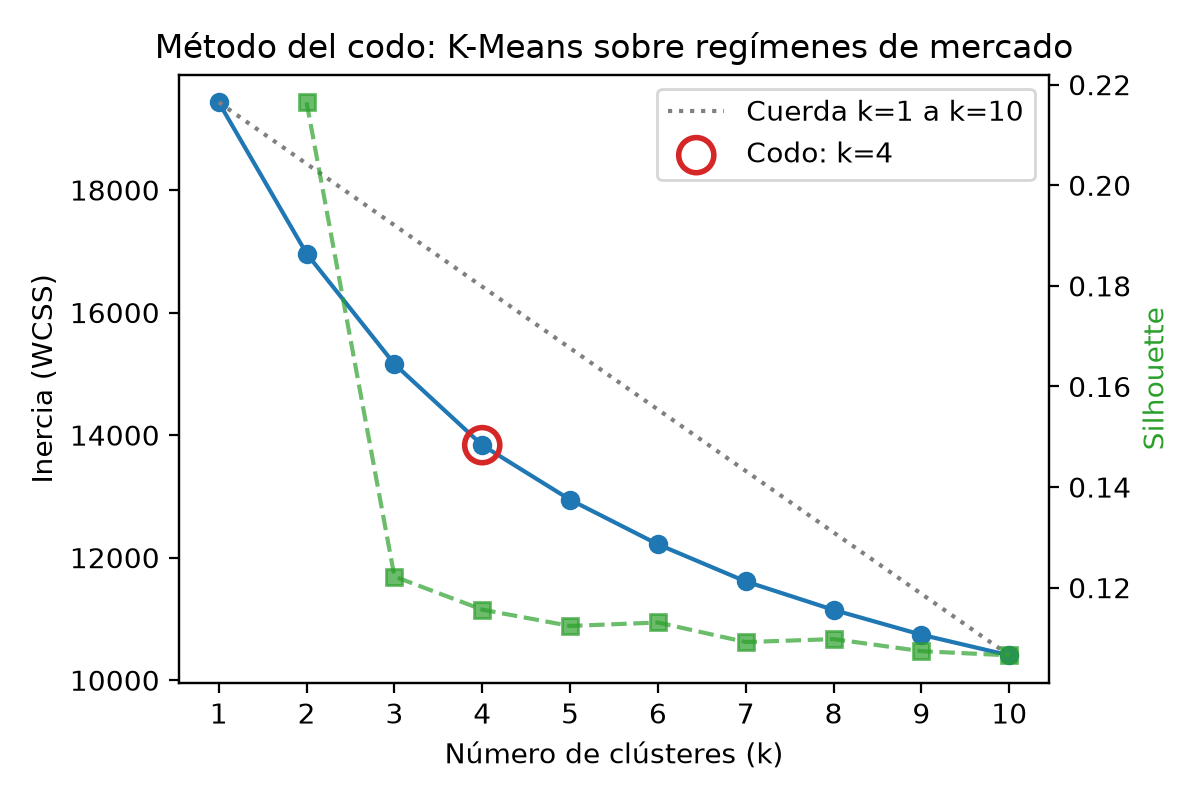
\includegraphics[width=\columnwidth]{codo_kmeans.png}
\caption{Método del codo: inercia y coeficiente de silueta para $k=1,\dots,10$.}
\label{fig:codo}
\end{figure}

\begin{figure}[t]
\centering
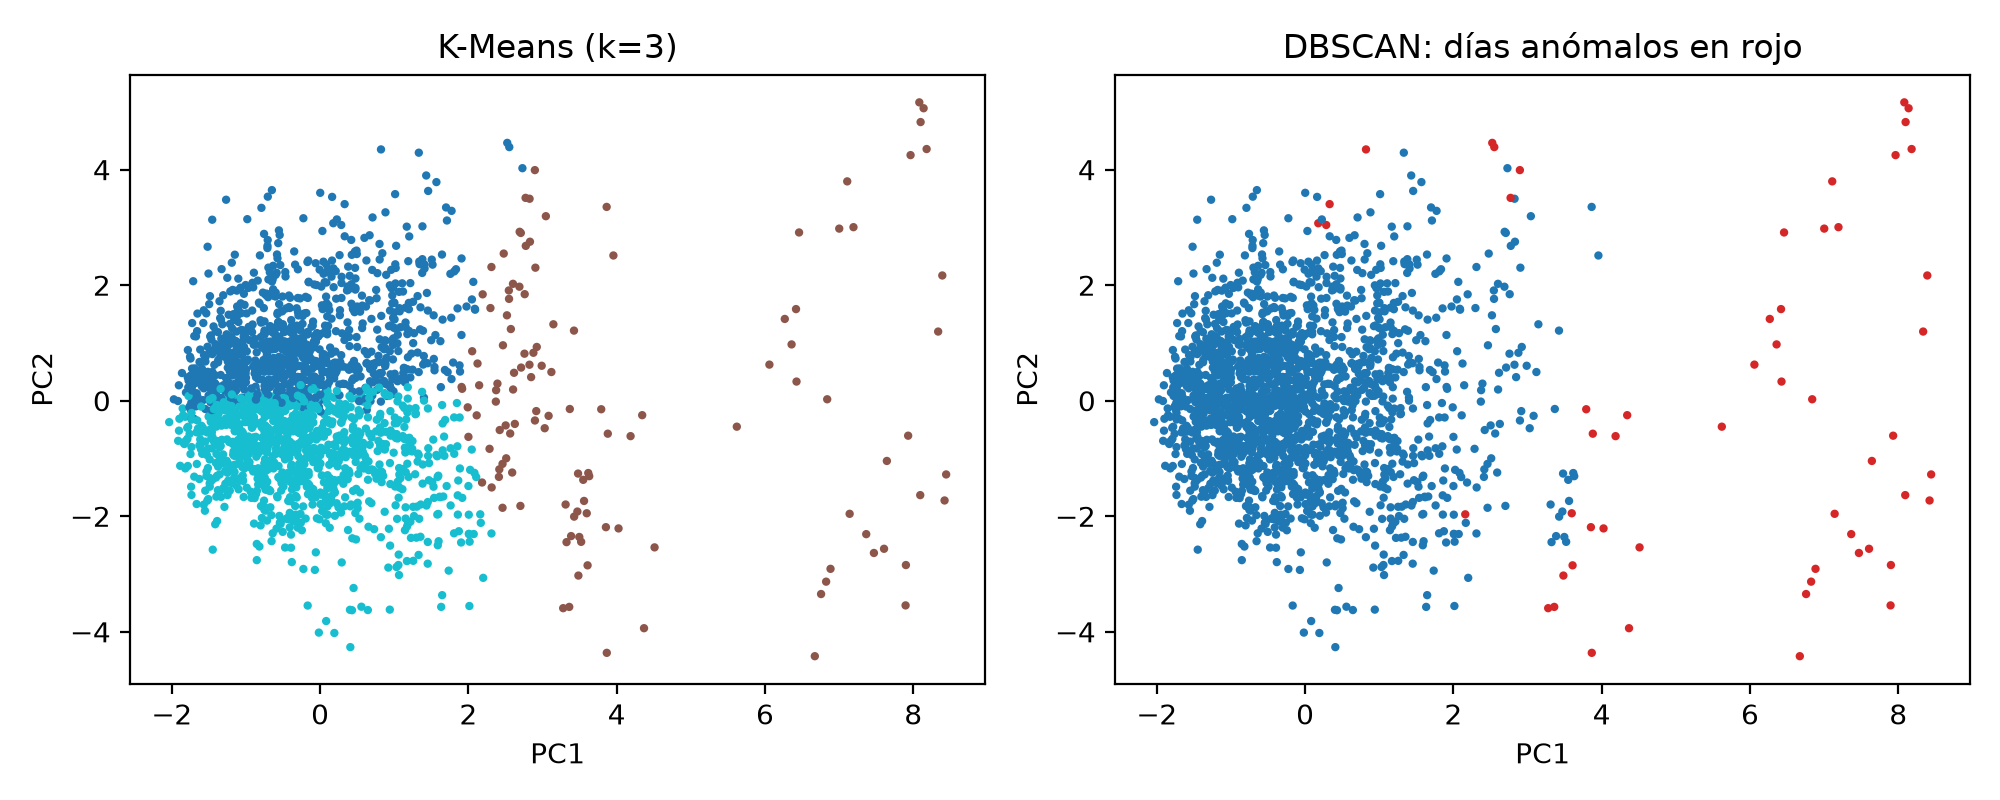
\includegraphics[width=0.95\columnwidth]{clusters_pca.png}
\caption{Proyección de los regímenes de mercado sobre los dos primeros componentes principales.}
\label{fig:pca}
\end{figure}

\subsubsection{Reglas de asociación}
Se discretizaron por terciles los retornos diarios de 8 mercados, junto con una bandera de alta volatilidad y la dirección siguiente de la TRM. Apriori~\cite{agrawal1994} y FP-Growth~\cite{han2000} (soporte mínimo de 0,05) producen los mismos 498 conjuntos frecuentes y 91 reglas cuyo consecuente es el sentido de la tasa de cambio (Tabla~\ref{tab:rules}), lo que valida ambas implementaciones entre sí. Los patrones coinciden con la teoría económica: un alza del Brent acompañada de una caída del DXY precede caídas de la TRM con confianza de 0,63 y lift de 1,22.

\begin{table}[t]
\caption{Reglas de asociación principales sobre la dirección de la TRM}
\label{tab:rules}
\centering
\footnotesize
\begin{tabular}{@{}p{4.3cm}p{0.8cm}rr@{}}
\toprule
Antecedente & TRM & Conf. & Lift \\
\midrule
USD/BRL sube, USD/MXN sube y VIX sube & sube & 0,60 & 1,24 \\
Brent sube, S\&P 500 sube y VIX baja & baja & 0,64 & 1,24 \\
S\&P 500 sube y USD/MXN sube & baja & 0,64 & 1,23 \\
Brent baja y hay alta volatilidad & sube & 0,59 & 1,23 \\
DXY sube, S\&P 500 baja y VIX sube & sube & 0,59 & 1,22 \\
Brent sube y DXY baja & baja & 0,63 & 1,22 \\
\bottomrule
\end{tabular}
\end{table}

\section{Módulo de Cloud Computing e Infraestructura}
La infraestructura corre en la nube pública de AWS, con región principal \texttt{us-east-1} y réplica de respaldo en \texttt{us-west-2} (Fig.~\ref{fig:arch}).

\subsection{Modelos de servicio y seguridad}
Según las definiciones del NIST~\cite{nist800145}, el diseño combina capas FaaS, PaaS, IaaS y SaaS (Tabla~\ref{tab:services}). De lunes a viernes a las 6:30~p.~m., una regla de EventBridge activa la función Lambda de ingesta, que consulta las APIs externas, corre el scraper y deja un archivo JSON en S3. La llegada de ese objeto dispara la Lambda de ETL, que limpia y carga la jornada en una base RDS PostgreSQL~16. Los modelos entrenados se guardan en S3 y los consume una aplicación FastAPI empaquetada en Docker, que corre en instancias EC2 repartidas en dos zonas de disponibilidad detrás de un Application Load Balancer (ALB).

En seguridad, la base de datos y la Lambda de ETL están en subredes privadas sin salida a Internet. RDS solo admite conexiones de los grupos de seguridad del ETL y de la API, y las instancias EC2 solo reciben tráfico del ALB. Terraform genera la contraseña de la base de datos y la guarda cifrada en SSM Parameter Store, los buckets de S3 bloquean el acceso público y el sistema no maneja datos personales.

\begin{table}[t]
\caption{Modelos de servicio en AWS y justificación técnica}
\label{tab:services}
\centering
\footnotesize
\begin{tabular}{@{}p{0.9cm}p{2.3cm}p{4.3cm}@{}}
\toprule
Modelo & Servicio & Justificación \\
\midrule
FaaS & Lambda + EventBridge & La ingesta y el ETL corren pocos segundos al día, con pago por ejecución \\
PaaS & RDS PostgreSQL 16 & Backups automáticos, parches y soporte Multi-AZ administrado \\
PaaS & S3, ECR y ALB & Almacenamiento duradero, registro Docker y balanceo administrado \\
IaaS & EC2 + Auto Scaling & Control de las instancias, las políticas de escalado y los chequeos de salud \\
SaaS & Tablero web FastAPI & Interfaz de consulta y simulación para el usuario final \\
\bottomrule
\end{tabular}
\end{table}

\subsection{Infraestructura como Código (Terraform)}
Todos los recursos se declaran en Terraform~\cite{terraform_aws} ($\geq 1.6$, proveedor AWS 5.x) dentro de \texttt{infra/terraform}, en 10 archivos que suman cerca de 980 líneas y 64 recursos administrados (Tabla~\ref{tab:iac}). Un \texttt{terraform apply} levanta la plataforma completa en unos 15 minutos y \texttt{terraform destroy} la elimina sin dejar residuos. Las variables permiten adaptar los permisos al rol \texttt{LabRole} de AWS Academy sin tocar la lógica.

El siguiente fragmento de \texttt{compute.tf} muestra la política de seguimiento de objetivo que mantiene el uso promedio de CPU en 60~\%:

{\scriptsize
\begin{verbatim}
resource "aws_autoscaling_policy" "cpu" {
  name = "${local.name}-cpu-target"
  autoscaling_group_name =
    aws_autoscaling_group.api.name
  policy_type = "TargetTrackingScaling"
  target_tracking_configuration {
    predefined_metric_specification {
      predefined_metric_type =
        "ASGAverageCPUUtilization"
    }
    target_value = var.cpu_target
  }
}
\end{verbatim}
}

\begin{table}[t]
\caption{Módulos de Infraestructura como Código en Terraform}
\label{tab:iac}
\centering
\footnotesize
\begin{tabular}{@{}p{1.9cm}p{5.7cm}@{}}
\toprule
Archivo & Recursos aprovisionados \\
\midrule
\texttt{network.tf} & VPC, subredes públicas y privadas en dos zonas, tablas de rutas, security groups y endpoint de S3 \\
\texttt{storage.tf} & Buckets de S3 con versionado, cifrado, ciclo de vida y réplica a us-west-2, y repositorio ECR \\
\texttt{database.tf} & RDS PostgreSQL 16 (db.t4g.micro, 20 GB), backups de 7 días y parámetros en SSM \\
\texttt{compute.tf} & Balanceador ALB, launch template, Auto Scaling Group (mínimo 2, máximo 4) y política de escalado \\
\texttt{lambda.tf} & Lambdas de ingesta y ETL, regla diaria de EventBridge y disparador desde S3 \\
\texttt{iam.tf} & Roles y permisos (o vínculo a LabRole en AWS Academy) \\
\texttt{monitoring.tf} & Tablero y 3 alarmas de CloudWatch, avisos SNS y presupuesto de 30 USD en AWS Budgets \\
\texttt{variables.tf}, \texttt{outputs.tf}, \texttt{versions.tf} & Variables de entrada, salidas y restricciones de versión \\
\bottomrule
\end{tabular}
\end{table}

\subsection{Escalabilidad, alta disponibilidad y recuperación}
Sobre el despliegue real en AWS se corrieron pruebas de fallo y de carga, registradas en \texttt{reports/experiments} (Tabla~\ref{tab:exp}). Se sondeó el endpoint \texttt{/health} cada medio segundo y se terminó de forma forzada una instancia EC2. Con un mínimo de una sola instancia hubo 109~s sin servicio (77,8~\% de disponibilidad). Con un mínimo de 2 instancias en zonas distintas, las 378 peticiones de prueba respondieron sin interrupciones (100~\%) mientras el grupo levantaba el nodo de reemplazo en 139~s (Fig.~\ref{fig:ha}).

En la prueba de carga, 16 clientes enviaron peticiones simultáneas a \texttt{/api/scenario} durante 14 minutos. Al superar el 60~\% de CPU, el auto-scaling subió de 2 a 4 instancias en el minuto 6,6 y quedaron listas en el minuto 9,2. En total se atendieron 4.543 solicitudes sin errores, la capacidad subió 84~\% y la latencia mediana bajó 60~\% (Fig.~\ref{fig:load}).

Para contingencias mayores se usa el esquema \emph{backup and restore}~\cite{aws_wellarchitected}: réplica de S3 en \texttt{us-west-2}, respaldos diarios de RDS con retención de 7 días y redespliegue con Terraform, con una pérdida máxima de 24 horas de datos (RPO) y restauración en menos de 1 hora (RTO).

\begin{table}[t]
\caption{Resultados de alta disponibilidad y pruebas de carga}
\label{tab:exp}
\centering
\footnotesize
\begin{tabular}{@{}lrrr@{}}
\toprule
\multicolumn{4}{@{}l}{\emph{Alta disponibilidad (terminación forzada de instancia)}} \\
Mínimo del grupo & Disponib. & Caída & Recuperación \\
\midrule
1 instancia & 77,8~\% & 109~s & --- \\
2 instancias & 100,0~\% & 0~s & 139~s \\
\midrule
\multicolumn{4}{@{}l}{\emph{Prueba de carga (16 clientes en \texttt{/api/scenario})}} \\
Instancias & Pet./s & p50 (s) & p95 (s) \\
\midrule
2 & 4,12 & 4,05 & 7,62 \\
4 & 7,59 & 1,61 & 4,87 \\
\bottomrule
\end{tabular}
\end{table}

\begin{figure}[t]
\centering
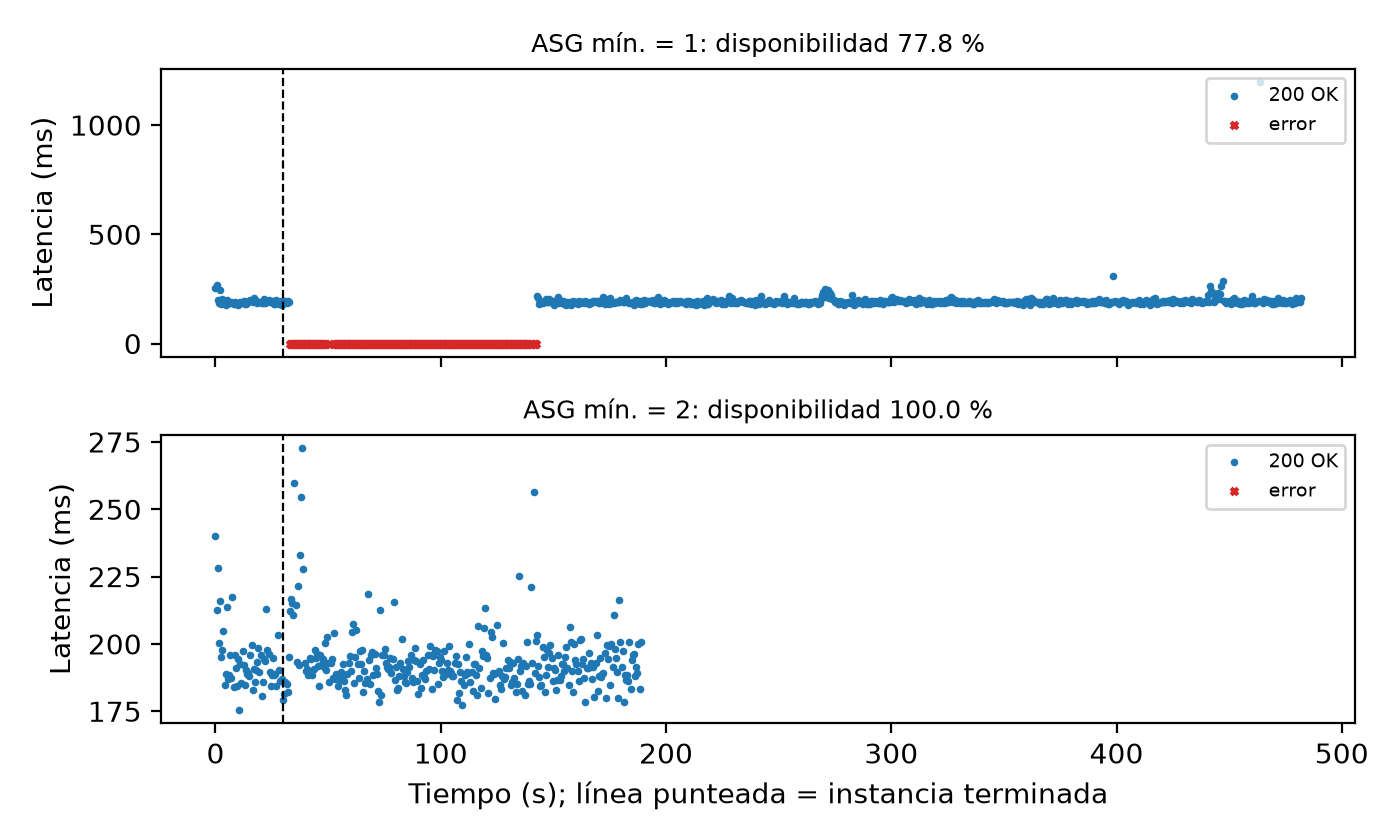
\includegraphics[width=\columnwidth]{ha_timeline.png}
\caption{Latencia de \texttt{/health} al terminar una instancia (mínimo de 1 frente a 2 instancias).}
\label{fig:ha}
\end{figure}

\begin{figure}[t]
\centering
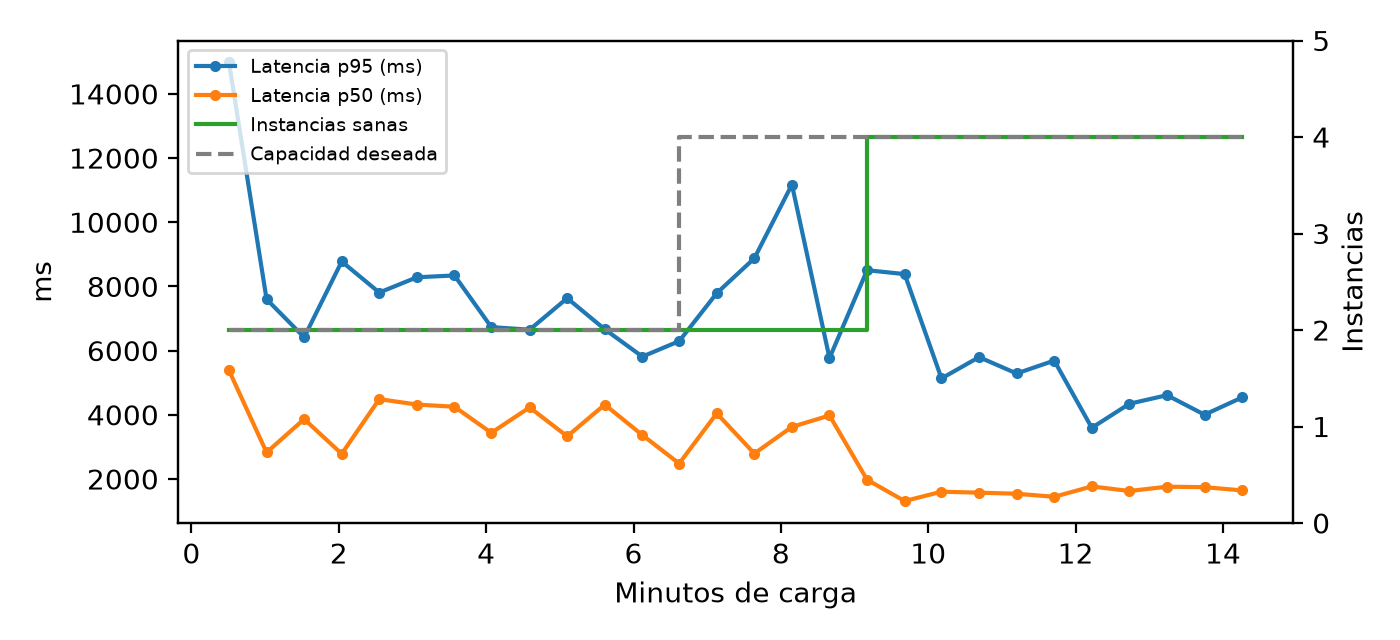
\includegraphics[width=\columnwidth]{load_timeline.png}
\caption{Comportamiento del auto-scaling bajo carga concurrente de 16 clientes.}
\label{fig:load}
\end{figure}

\subsection{Estimación preliminar de costos}
Con tarifas on-demand de \texttt{us-east-1} y 730 horas al mes (\texttt{docs/costos.md}), operar la arquitectura sin apagarla cuesta alrededor de 63,6~USD al mes (Tabla~\ref{tab:cost}), valor que subiría a entre 78 y 95~USD con Multi-AZ activo y 4 nodos. Como Terraform permite encender el entorno solo durante las sesiones de integración, pruebas y sustentación, el gasto proyectado para todo el semestre es de unos 21~USD (Tabla~\ref{tab:sem}), cubierto por los créditos de AWS Academy y vigilado con un presupuesto de 30~USD con alertas al 50~\%, 80~\% y 100~\%. El ahorro principal viene de reemplazar el NAT Gateway por un endpoint de S3 (unos 33~USD menos al mes), usar Lambda para la ingesta diaria, elegir instancias pequeñas (\texttt{t3.micro} y \texttt{db.t4g.micro}) y activar Multi-AZ solo durante la demostración (unos 14~USD menos al mes).

\begin{table}[t]
\caption{Costo mensual estimado (USD, on-demand, us-east-1, 24/7)}
\label{tab:cost}
\centering
\footnotesize
\begin{tabular}{@{}p{2.6cm}p{3.5cm}r@{}}
\toprule
Servicio & Configuración & USD/mes \\
\midrule
Application Load Balancer & 1 ALB con tráfico bajo & 17,0 \\
EC2 & 2 instancias t3.micro & 15,2 \\
EBS & 2 discos gp3 de 8 GB & 1,3 \\
Direcciones IPv4 públicas & 4 direcciones asociadas & 14,6 \\
RDS PostgreSQL & db.t4g.micro en una zona & 11,7 \\
Almacenamiento de RDS & 20 GB gp3 & 2,3 \\
S3 con réplica y ECR & Menos de 1 GB & 0,2 \\
Lambda, EventBridge y SSM & Unas 44 ejecuciones al mes & 0,0 \\
CloudWatch & 1 tablero, 3 alarmas y logs & 0,8 \\
Transferencia de datos & Menos de 5 GB & 0,5 \\
\midrule
\textbf{Total} & & \textbf{63,6} \\
\bottomrule
\end{tabular}
\end{table}

\begin{table}[t]
\caption{Costo esperado del semestre}
\label{tab:sem}
\centering
\footnotesize
\begin{tabular}{@{}lrr@{}}
\toprule
Etapa & Horas encendido & USD \\
\midrule
Desarrollo e integración & 40 & 3,5 \\
Pruebas de auto-scaling y failover & 24 & 2,5 \\
Semana de sustentación & 168 & 14,6 \\
\midrule
\textbf{Total} & & $\approx$ \textbf{21,0} \\
\bottomrule
\end{tabular}
\end{table}

\section{Integración con Machine Learning}
Como el proyecto integra también la asignatura de Machine Learning, en esta sección se documenta ese componente, que ya está implementado en \texttt{src/pipeline/train.py} y cuyos resultados están en \texttt{reports/model\_results.json}.
\subsection{Diseño experimental}
Los datos se dividieron cronológicamente: entrenamiento de sep.~2017 a dic.~2024 (1.727 días) y prueba de dic.~2024 a oct.~2026 (432 días). Dentro del entrenamiento, los hiperparámetros se optimizaron con \texttt{TimeSeriesSplit} de 5 pliegues, de modo que cada pliegue de validación queda después de su pliegue de entrenamiento. Todos los modelos son pipelines de scikit-learn~\cite{pedregosa2011}. Candidatos de regresión: lineal, polinomial (grado 2 sobre las $k$ mejores variables) + Ridge, Ridge, Lasso, Elastic Net, Random Forest~\cite{breiman2001} y Gradient Boosting~\cite{friedman2001}. Candidatos de clasificación (para dirección y riesgo): regresión logística, KNN, SVM (RBF), Random Forest, AdaBoost~\cite{freund1997} y Gradient Boosting. Se usó Grid Search en los espacios de baja dimensión (modelos lineales, KNN, SVM, AdaBoost) y Random Search~\cite{bergstra2012} con 15 muestras para los ensembles. Los modelos finales se eligen por el puntaje de validación cruzada, nunca por el de prueba.

\subsection{Resultados}
Las Tablas~\ref{tab:clf} y~\ref{tab:reg} reportan las métricas de prueba. En la clasificación de dirección, los modelos lineales, KNN y SVM quedan en el nivel del azar o por debajo (AUC 0,47--0,50), aunque su AUC en validación cruzada rondaba 0,56: su señal aparente no sobrevivió al cambio de periodo. Solo los ensembles conservan una ventaja (AUC 0,54--0,57), lo que indica interacciones no lineales entre los determinantes. El mismo patrón se observa en riesgo (AUC de hasta 0,586) y en regresión, donde Gradient Boosting reduce en 2,4~\% el RMSE del paseo aleatorio y Random Forest logra un acierto direccional del 54,6~\%. La exactitud en dirección con umbral 0,5 (53,2~\%) aún está por debajo de la clase mayoritaria (54,6~\%, un periodo en el que el peso se apreció), una limitación que se explica porque el periodo de prueba estuvo dominado por la apreciación del peso.

\begin{table}[t]
\caption{Resultados de prueba: clasificación (432 días)}
\label{tab:clf}
\centering
\footnotesize
\begin{tabular}{@{}lccccc@{}}
\toprule
 & \multicolumn{3}{c}{Dirección} & \multicolumn{2}{c}{Riesgo} \\
\cmidrule(lr){2-4}\cmidrule(l){5-6}
Modelo & AUC VC & AUC & Exact. & AUC VC & AUC \\
\midrule
Logística & 0,559 & 0,497 & 0,519 & 0,599 & 0,549 \\
KNN & 0,565 & 0,474 & 0,486 & 0,597 & 0,571 \\
SVM & 0,557 & 0,490 & 0,484 & 0,595 & 0,562 \\
Random Forest & \textbf{0,582} & 0,555 & 0,532 & \textbf{0,623} & 0,585 \\
AdaBoost & 0,562 & 0,541 & 0,521 & 0,600 & 0,557 \\
Gradient Boost. & 0,578 & \textbf{0,566} & 0,532 & 0,615 & \textbf{0,586} \\
\midrule
Línea base & -- & 0,500 & 0,546 & -- & 0,500 \\
\bottomrule
\end{tabular}
\end{table}

\begin{table}[t]
\caption{Resultados de prueba: regresión del siguiente retorno}
\label{tab:reg}
\centering
\footnotesize
\begin{tabular}{@{}lcccc@{}}
\toprule
Modelo & RMSE (\%) & RMSE/PA & $R^2$ & Acierto dir. \\
\midrule
Paseo aleatorio & 0,769 & 1,000 & -- & -- \\
Lineal & 0,772 & 1,005 & $-0{,}019$ & 0,509 \\
Poli(2)+Ridge & 0,764 & 0,993 & 0,004 & 0,500 \\
Ridge & 0,767 & 0,997 & $-0{,}004$ & 0,493 \\
Lasso & 0,765 & 0,995 & 0,000 & 0,502 \\
Elastic Net & 0,765 & 0,994 & 0,002 & 0,491 \\
Random Forest & 0,759 & 0,987 & 0,017 & \textbf{0,546} \\
Gradient Boost. & \textbf{0,751} & \textbf{0,976} & \textbf{0,038} & 0,542 \\
\bottomrule
\end{tabular}
\end{table}

\subsection{Interpretabilidad}
TreeSHAP sobre el modelo de dirección Random Forest (Fig.~\ref{fig:shap}) ubica en primer lugar la brecha spot--TRM: cuando la última cotización spot está por encima de la TRM vigente, la siguiente TRM tiende a subir, lo que refleja que la TRM promedia las operaciones del día. Le siguen el último retorno de la TRM, la variación diaria del DXY y del dólar spot y el retorno a 5 días del Brent. La importancia por impureza coincide en cuatro de las cinco primeras variables (brecha spot--TRM, último retorno de la TRM y variaciones diarias del USD/COP y del DXY). LIME sobre el último día de prueba da una explicación local: el alza del 5~\% del Brent en cinco días y la caída del 1~\% del dólar spot el día anterior reducen la probabilidad de alza, mientras que la brecha spot--TRM y el último retorno de la TRM la aumentan. Es una explicación legible que puede mostrarse junto a cada pronóstico.

\begin{figure}[t]
\centering
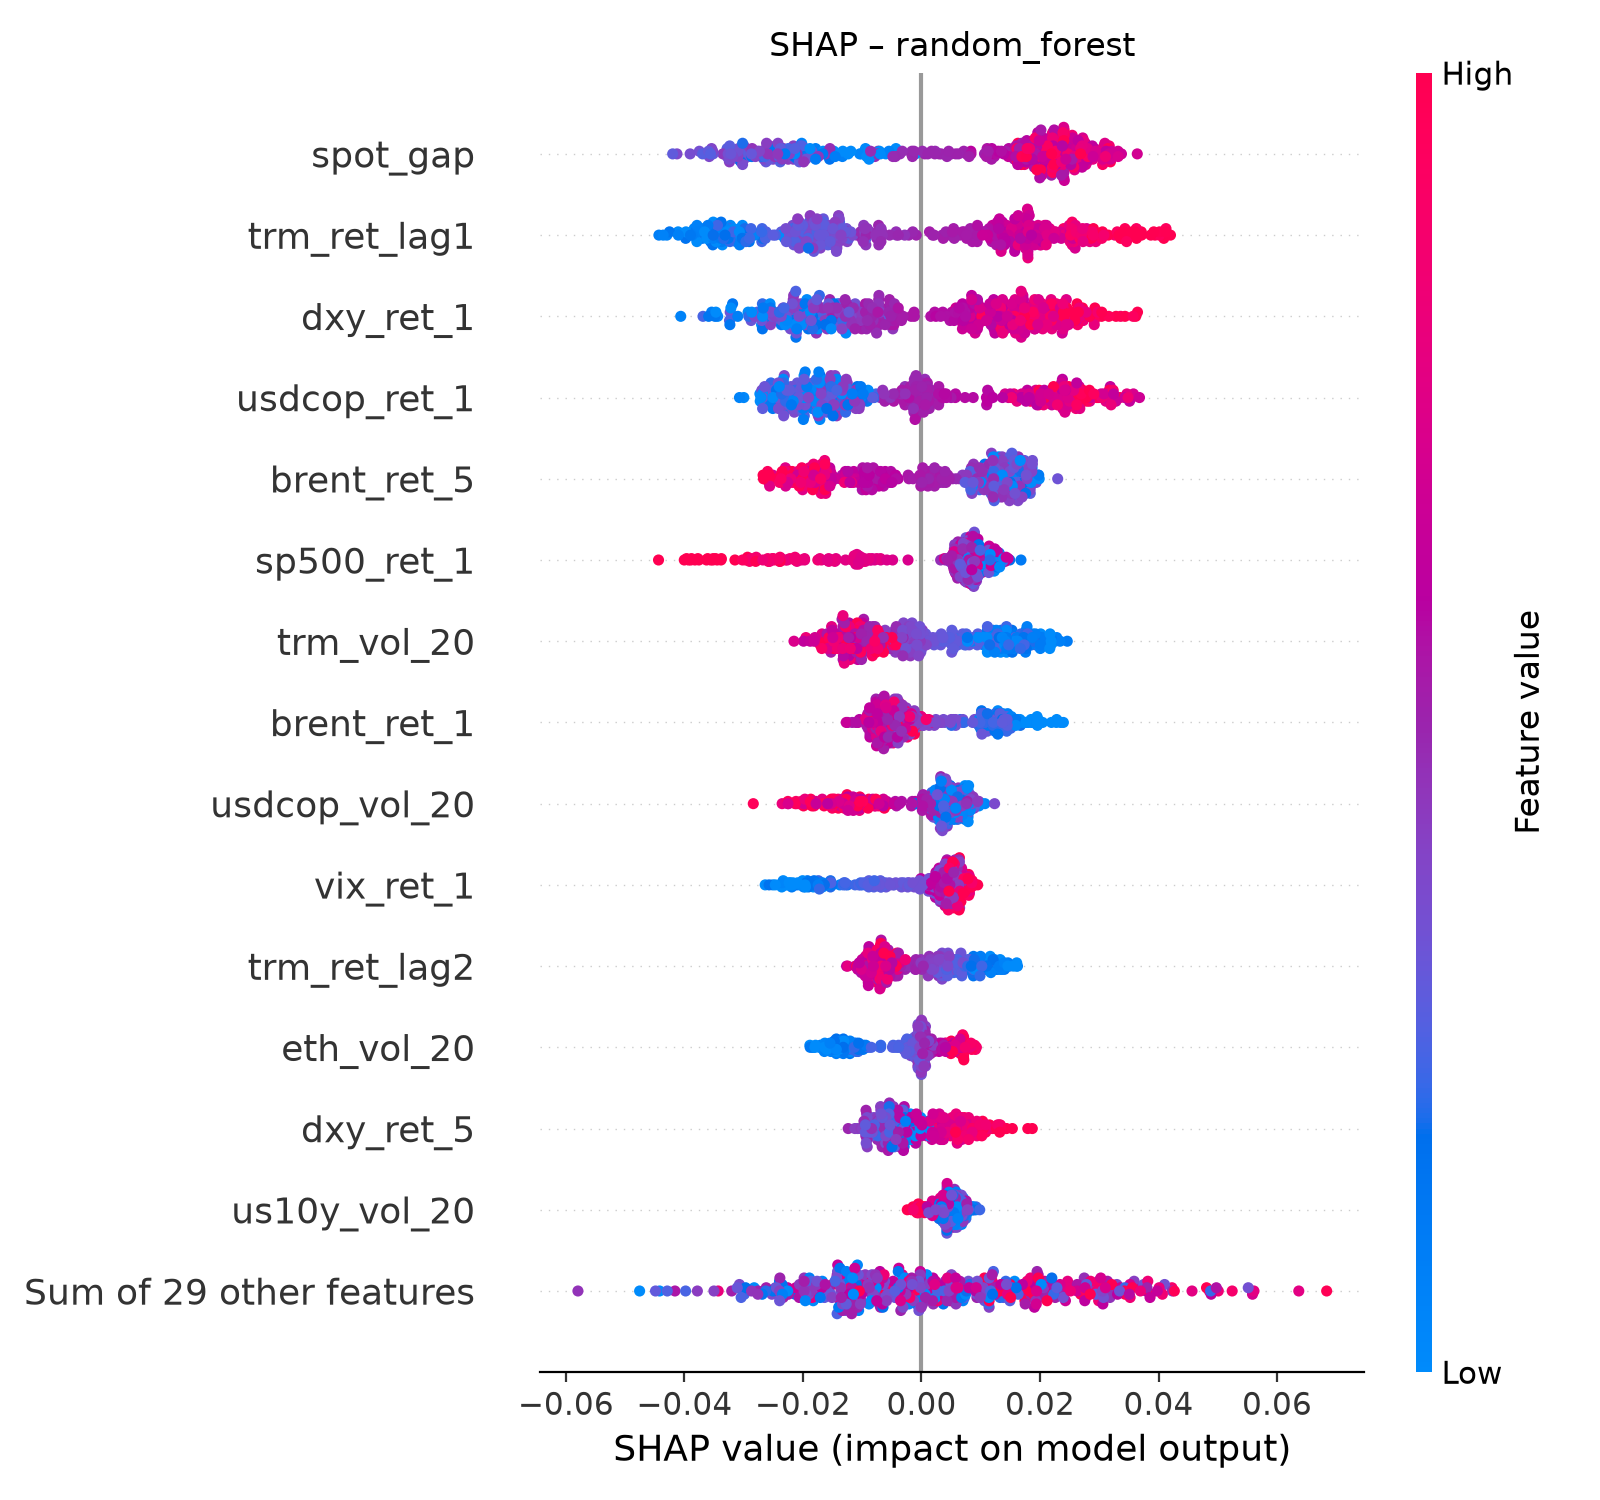
\includegraphics[width=0.92\columnwidth]{shap_beeswarm.png}
\caption{Valores SHAP del modelo de dirección Random Forest en el conjunto de prueba.}
\label{fig:shap}
\end{figure}

\subsection{Evaluación orientada a decisiones}
Las métricas estadísticas no dicen si el modelo ayuda a un usuario. Simulamos un hogar que recibe USD~1.000 al día y vende a la TRM vigente, o espera un día cuando $P(\text{sube})>\tau$. En el periodo de prueba (Fig.~\ref{fig:backtest}), la regla con Random Forest y $\tau=0{,}5$ gana en promedio 383 COP al día frente a vender siempre de inmediato, y 624 COP con $\tau=0{,}55$; con Gradient Boosting gana 495 y 1.832 COP, respectivamente. Decidir al azar entre vender o esperar \emph{pierde} 1.383 COP al día, porque el peso se apreció durante el periodo de prueba, y un oráculo perfecto ganaría 9.994 COP. Las ganancias son pequeñas pero positivas y robustas al umbral. Para la alerta de riesgo, un umbral de probabilidad elegido en el último pliegue de entrenamiento, de modo que la tasa de alertas iguale la frecuencia histórica, logra en prueba una precisión del 30,1~\% frente a una tasa base del 22,5~\% (lift 1,34), con una exhaustividad del 25,8~\%. Las probabilidades del Random Forest están algo mejor calibradas que la tasa base (Brier 0,247 frente a 0,249).

\begin{figure}[t]
\centering
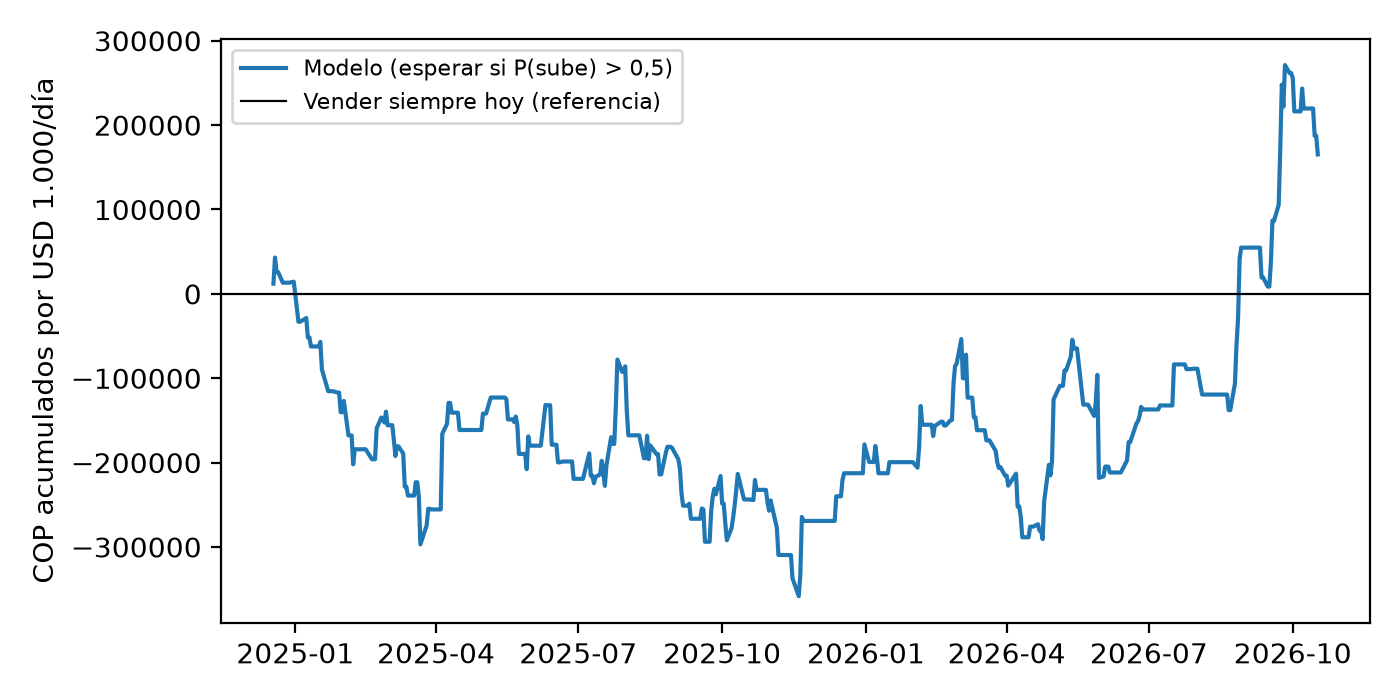
\includegraphics[width=\columnwidth]{decision_backtest.png}
\caption{Ganancia acumulada de la regla del hogar con remesas (Random Forest, $\tau=0{,}5$) frente a vender siempre de inmediato.}
\label{fig:backtest}
\end{figure}

\subsection{Selección del modelo}
Se eligió Random Forest para dirección, riesgo y regresión porque obtiene el mejor puntaje de validación cruzada en dos de las tres tareas, nunca queda lejos del mejor resultado de prueba y una sola familia de modelos simplifica el mantenimiento y la explicación. La búsqueda aleatoria de cada ensemble tarda de 60 a 77~s en un portátil, y servir los tres modelos toma cerca de 0,5~s por petición en una \texttt{t3.micro}. Gradient Boosting se conserva como alternativa documentada, pues obtuvo puntajes de prueba ligeramente mejores.

\subsection{Acople con Minería de Datos y Cloud}
Los dos módulos anteriores son la base del modelado. La matriz de 43 variables sin fuga de información (\texttt{dataset.csv}) y las etiquetas de régimen de K-Means alimentan los tres objetivos: dirección (\texttt{y\_up}), retorno esperado (\texttt{y\_ret}) y riesgo de movimiento fuerte. Los modelos entrenados (\texttt{src/pipeline/train.py}) se serializan y versionan en S3; cuando un contenedor arranca en EC2, la API FastAPI descarga el artefacto vigente y atiende \texttt{/api/predict} y \texttt{/api/scenario}, junto con consultas históricas a RDS para el tablero web (Fig.~\ref{fig:dash}).

\begin{figure}[t]
\centering
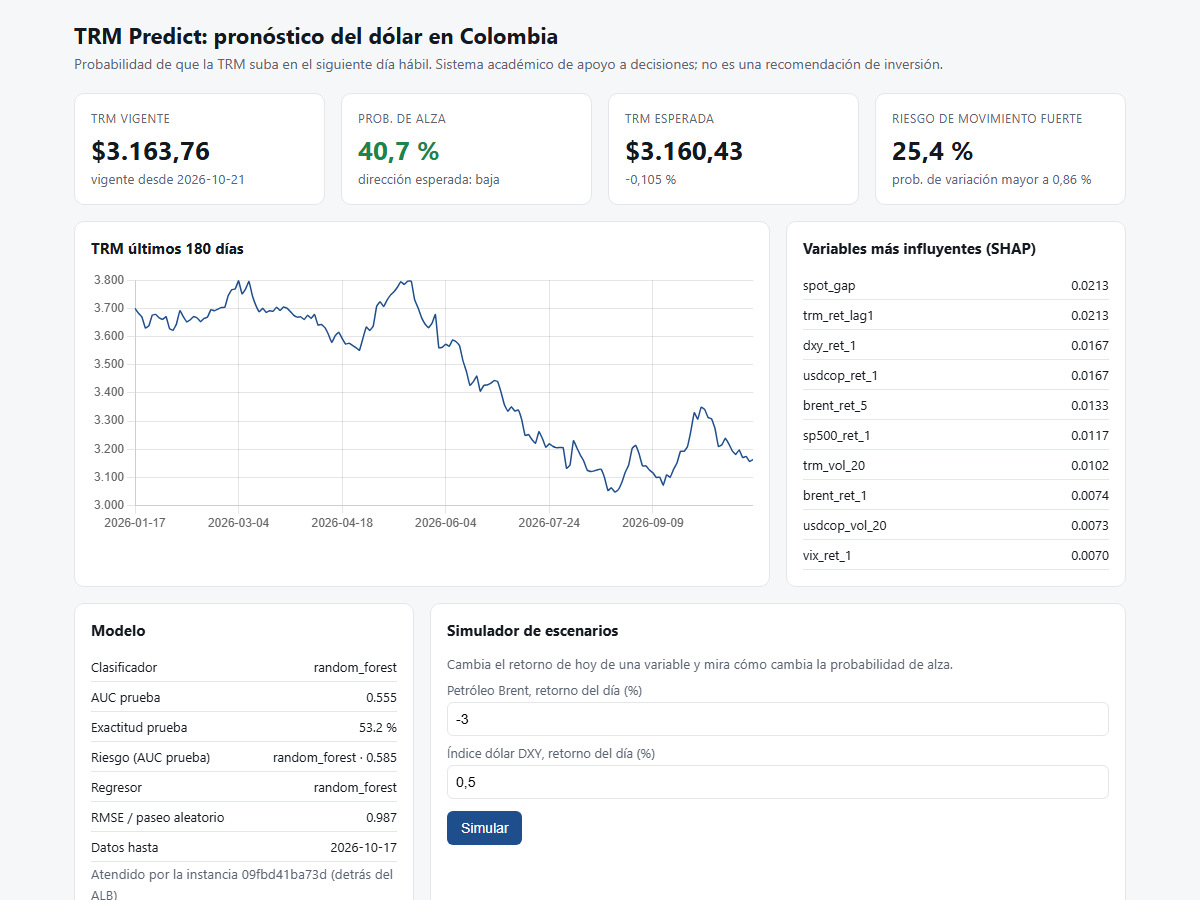
\includegraphics[width=\columnwidth]{tablero_aws.png}
\caption{Tablero servido desde AWS: TRM vigente, probabilidad de alza, TRM esperada, riesgo de movimiento fuerte, variables SHAP y simulador de escenarios.}
\label{fig:dash}
\end{figure}

\section{Reproducibilidad y repositorio}
Todo el código, la infraestructura y los resultados están versionados en el repositorio oficial~\cite{repo}. La ingesta está en \texttt{src/ingest/} (\texttt{apis.py} y \texttt{scraper.py}); la preparación (\texttt{prepare.py}), el EDA (\texttt{eda.py}), la minería no supervisada (\texttt{unsupervised.py}, \texttt{elbow.py}, \texttt{kmeans\_validation.py}) y el entrenamiento (\texttt{train.py}) están en \texttt{src/pipeline/}; Terraform está en \texttt{infra/terraform/}, y los registros de calidad, las pruebas en la nube y las figuras quedan en \texttt{reports/}. El pipeline se reproduce con:

{\scriptsize
\begin{verbatim}
pip install -r requirements.txt
python -m src.ingest.run
python -m src.pipeline.prepare
python -m src.pipeline.eda
python -m src.pipeline.unsupervised
python -m src.pipeline.train
cd infra/terraform && terraform init
terraform apply
\end{verbatim}
}

Las semillas aleatorias están fijas y los datos crudos descargados se incluyen en \texttt{data/raw/}, de modo que las tablas y figuras de este documento se pueden regenerar sin depender de la disponibilidad de las APIs.

\section{Trabajo pendiente para la entrega final}
Antes de la entrega final del 26 de noviembre de 2026 quedan cuatro tareas: (i) contrastar la factura real de AWS Cost Explorer con la Tabla~\ref{tab:cost}; (ii) hacer una prueba controlada de failover en RDS con Multi-AZ activo; (iii) incorporar al entrenamiento el histórico acumulado del índice de sentimiento de noticias; y (iv) consolidar la versión en inglés del reporte (\texttt{docs/reporte/report\_en.tex}) y dejar el entorno desplegado durante la semana de sustentación con el enlace del tablero activo.

\begin{thebibliography}{99}
\bibitem{banrep_remesas} Banco de la Rep\'ublica de Colombia, ``Ingresos de remesas de trabajadores en Colombia,'' Estad\'isticas del sector externo, 2025. [En línea]. Disponible: \url{https://www.banrep.gov.co}
\bibitem{un2015} United Nations, ``Transforming our world: The 2030 Agenda for Sustainable Development,'' A/RES/70/1, 2015.
\bibitem{meese1983} R. A. Meese and K. Rogoff, ``Empirical exchange rate models of the seventies: Do they fit out of sample?'' \emph{J. Int. Econ.}, vol. 14, no. 1--2, pp. 3--24, 1983.
\bibitem{henrique2019} B. M. Henrique, V. A. Sobreiro, and H. Kimura, ``Literature review: Machine learning techniques applied to financial market prediction,'' \emph{Expert Syst. Appl.}, vol. 124, pp. 226--251, 2019.
\bibitem{sezer2020} O. B. Sezer, M. U. Gudelek, and A. M. Ozbayoglu, ``Financial time series forecasting with deep learning: A systematic literature review: 2005--2019,'' \emph{Appl. Soft Comput.}, vol. 90, Art. no. 106181, 2020.
\bibitem{lundberg2017} S. M. Lundberg and S.-I. Lee, ``A unified approach to interpreting model predictions,'' in \emph{Adv. Neural Inf. Process. Syst. (NeurIPS)}, vol. 30, 2017, pp. 4765--4774.
\bibitem{ribeiro2016} M. T. Ribeiro, S. Singh, and C. Guestrin, ```Why should I trust you?': Explaining the predictions of any classifier,'' in \emph{Proc. 22nd ACM SIGKDD Int. Conf. Knowl. Discov. Data Min.}, 2016, pp. 1135--1144.
\bibitem{fayyad1996} U. Fayyad, G. Piatetsky-Shapiro, and P. Smyth, ``From data mining to knowledge discovery in databases,'' \emph{AI Mag.}, vol. 17, no. 3, pp. 37--54, 1996.
\bibitem{wirth2000} R. Wirth and J. Hipp, ``CRISP-DM: Towards a standard process model for data mining,'' in \emph{Proc. 4th Int. Conf. Pract. Appl. Knowl. Discov. Data Min.}, 2000, pp. 29--39.
\bibitem{ester1996} M. Ester, H.-P. Kriegel, J. Sander, and X. Xu, ``A density-based algorithm for discovering clusters in large spatial databases with noise,'' in \emph{Proc. 2nd Int. Conf. Knowl. Discov. Data Min. (KDD)}, 1996, pp. 226--231.
\bibitem{agrawal1994} R. Agrawal and R. Srikant, ``Fast algorithms for mining association rules,'' in \emph{Proc. 20th Int. Conf. Very Large Data Bases (VLDB)}, 1994, pp. 487--499.
\bibitem{han2000} J. Han, J. Pei, and Y. Yin, ``Mining frequent patterns without candidate generation,'' in \emph{Proc. ACM SIGMOD Int. Conf. Manag. Data}, 2000, pp. 1--12.
\bibitem{pedregosa2011} F. Pedregosa \emph{et al.}, ``Scikit-learn: Machine learning in Python,'' \emph{J. Mach. Learn. Res.}, vol. 12, pp. 2825--2830, 2011.
\bibitem{breiman2001} L. Breiman, ``Random forests,'' \emph{Mach. Learn.}, vol. 45, no. 1, pp. 5--32, 2001.
\bibitem{friedman2001} J. H. Friedman, ``Greedy function approximation: A gradient boosting machine,'' \emph{Ann. Statist.}, vol. 29, no. 5, pp. 1189--1232, 2001.
\bibitem{freund1997} Y. Freund and R. E. Schapire, ``A decision-theoretic generalization of on-line learning and an application to boosting,'' \emph{J. Comput. Syst. Sci.}, vol. 55, no. 1, pp. 119--139, 1997.
\bibitem{bergstra2012} J. Bergstra and Y. Bengio, ``Random search for hyper-parameter optimization,'' \emph{J. Mach. Learn. Res.}, vol. 13, pp. 281--305, 2012.
\bibitem{nist800145} P. Mell and T. Grance, ``The NIST definition of cloud computing,'' NIST, Gaithersburg, MD, USA, Special Publication 800-145, 2011.
\bibitem{terraform_aws} HashiCorp, ``Terraform AWS provider documentation,'' 2026. [En línea]. Disponible: \url{https://registry.terraform.io/providers/hashicorp/aws/latest/docs}
\bibitem{aws_wellarchitected} Amazon Web Services, ``Disaster recovery of workloads on AWS: Recovery in the cloud,'' AWS Whitepaper, 2021. [En línea]. Disponible: \url{https://docs.aws.amazon.com/whitepapers/latest/disaster-recovery-workloads-on-aws/}
\bibitem{repo} S. Cubides, N. Vergara, and E. Ruiz, ``TRM Predict,'' repositorio GitHub, 2026. [En línea]. Disponible: \url{https://github.com/Sebas-409/proyecto-integrador-trm}
\end{thebibliography}

\end{document}

